\documentclass[12pt]{article}

\usepackage[utf8]{inputenc}
\usepackage[T1]{fontenc}
\usepackage{datetime}
\usepackage[spanish]{babel}
\usepackage{graphicx}
\usepackage{listings}
\usepackage{caption}
\usepackage{subcaption}
\usepackage[right=2cm,left=2cm,top=2cm,bottom=2cm]{geometry}
\usepackage{hyperref}
\usepackage{fancyhdr}
\usepackage{color}
\usepackage[export]{adjustbox}
\usepackage{graphicx}
\usepackage{float}
\usepackage{changepage}
\usepackage{multicol}
\usepackage{imakeidx}
\usepackage{csquotes}
\usepackage{array}
\usepackage{tabularx}
\usepackage{xcolor}
\usepackage[backend=biber]{biblatex}
\addbibresource{webgrafia.bib}

\pagestyle{fancy}
\renewcommand{\footrulewidth}{0.4pt}
\setlength{\headheight}{15pt}


\fancyhead[L]{ CEIABD – MIA }
\fancyhead[R]{López, Marta Urbano – Páez Anguita, Víctor }
\fancyfoot[L]{IES Gran Capitán}

\begin{document}

\begin{titlepage}
    \begin{center}
      \Large \bfseries{}
    \end{center}
    \vspace{0.1cm}
    \begin{center}
      \Large \bfseries{}
    \end{center}
    \vspace{0.1cm}
    \begin{center}
     \Large \bfseries{Proyecto ChatBot}
    \end{center}
    \vspace{0.0001cm}
    \begin{center}
        Departamento de informática \\ I.E.S. Gran Capitán - Córdoba
    \end{center}
        \vspace{2 cm}
\begin{figure}[h!]
    \centering
    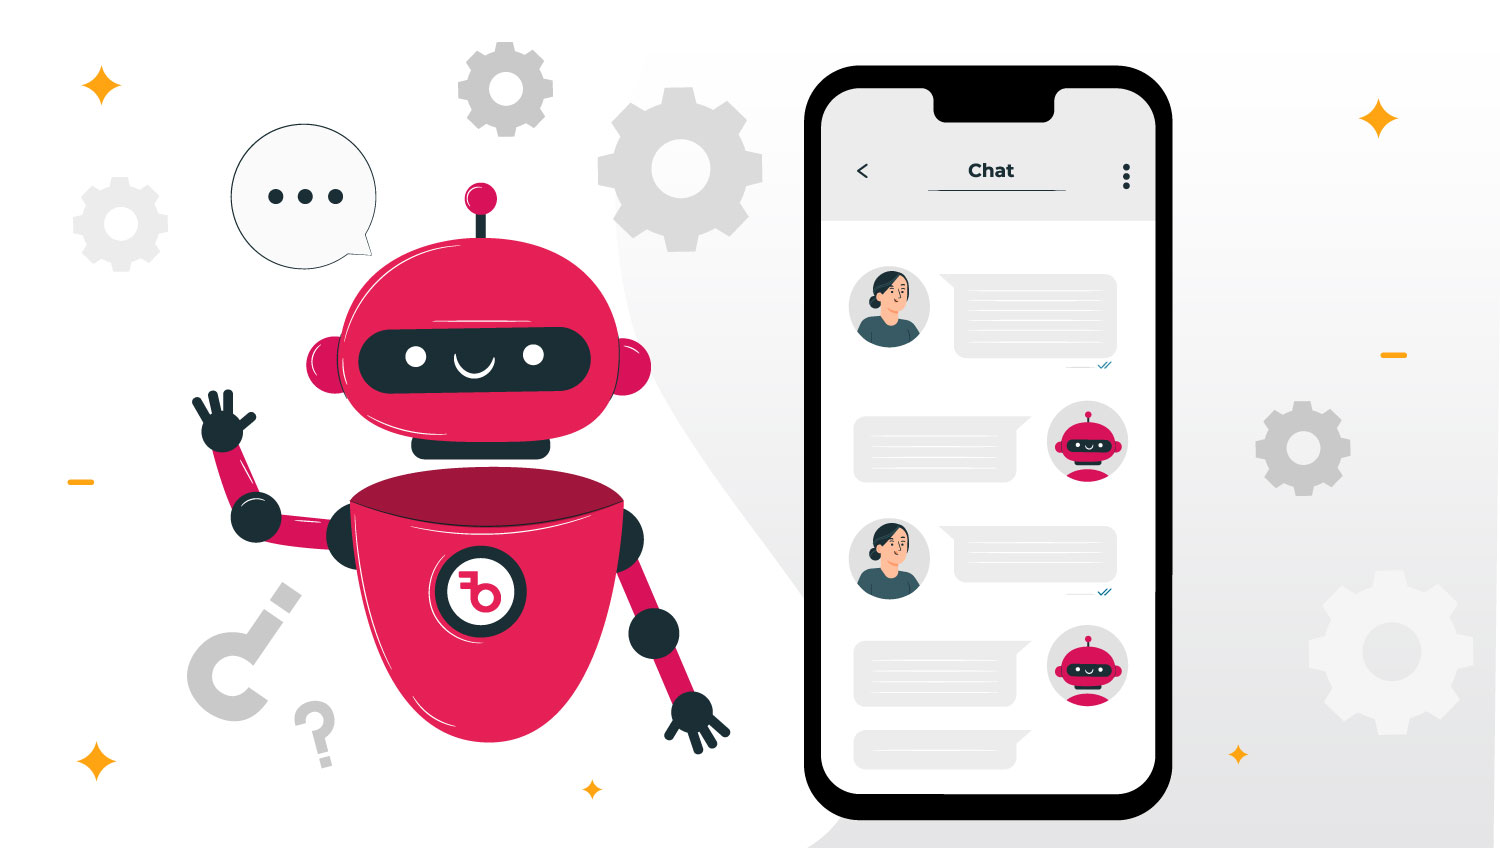
\includegraphics[width=.6\textwidth]{assets/portada.jpg}
    \label{fig:my_label}
\end{figure}
    \vspace{0.2 cm}
    \begin{center}
        Inteligencia artificial y Big data \\ \today 
    \end{center}
    \vspace{4 cm}
\null\hfill \textbf{Desarrollado por:}
\\
\\
\null\hfill Marta López Urbano
\\
\null\hfill Víctor Páez Anguita
\clearpage
\end{titlepage}

%%%%%%%%%%%%%%%%%%%%%%%%%%%Index%%%%%%%%%%%%%%%%%%%%%%%%%%%%%%%%
\tableofcontents
\clearpage
%%%%%%%%%%%%%%%%%%%%%%%%%%%Index%%%%%%%%%%%%%%%%%%%%%%%%%%%%%%%%


\section{Introducción}

En este documento se presenta el desarrollo de un chatbot utilizando Botpress, diseñado específicamente para asistir a los clientes de un 
hotel. El chatbot es capaz de gestionar reservas, proporcionar asistencia en problemas, sugerir actividades y contactar con soporte humano 
si es necesario. Se explicarán los diferentes aspectos técnicos trabajados en Botpress, como el flujo conversacional, 
las variables del chat, los prompts dinámicos y la integración con Booking para la verificación de reservas.

\section{Estructura del Chatbot en Botpress}

El desarrollo del chatbot en Botpress se ha basado en varios componentes fundamentales que permiten su correcto funcionamiento y su capacidad de 
respuesta eficiente.

\subsection{Flujo Conversacional}

El chatbot utiliza un workflow estructurado en Botpress que define los diferentes estados de la conversación. Este flujo permite dirigir al usuario 
a través de distintos procesos, empezando por la gestión de reservas y continuando con la decisión de actividades y la resolución de problemas.
Se han diseñado nodos de decisión que permiten personalizar la interacción según las necesidades del usuario.

\begin{figure}[h!]
    \centering
    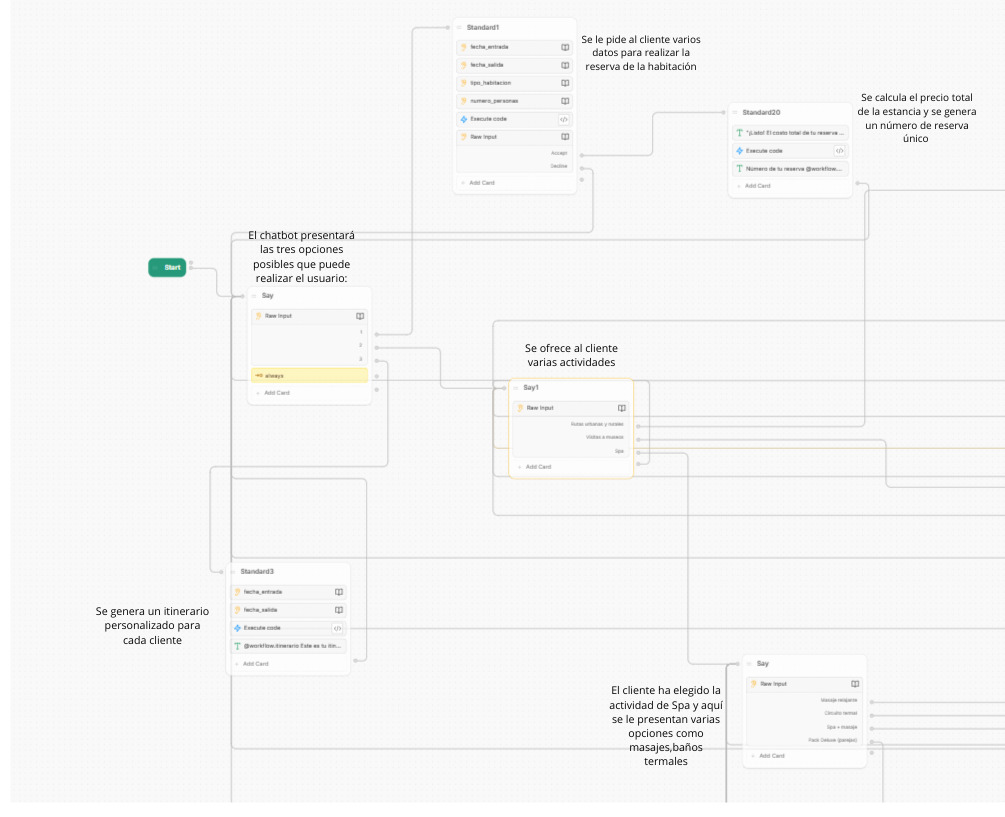
\includegraphics[width=.5\textwidth]{assets/workflow1.jpeg}
    \label{fig:my_label}
\end{figure}

Como podemos observar en el principio del flujo conversacional, el chatbot comienza saludando al usuario y ofreciendo ayuda para gestionar reservas.
A continuación, el chatbot pregunta al usuario si desea reservar una habitación o si necesita ayuda con otro tema. Dependiendo de la respuesta del usuario,
el chatbot dirige la conversación hacia la gestión de reservas o hacia otros temas como actividades o problemas.

\clearpage

\begin{figure}[h!]
    \centering
    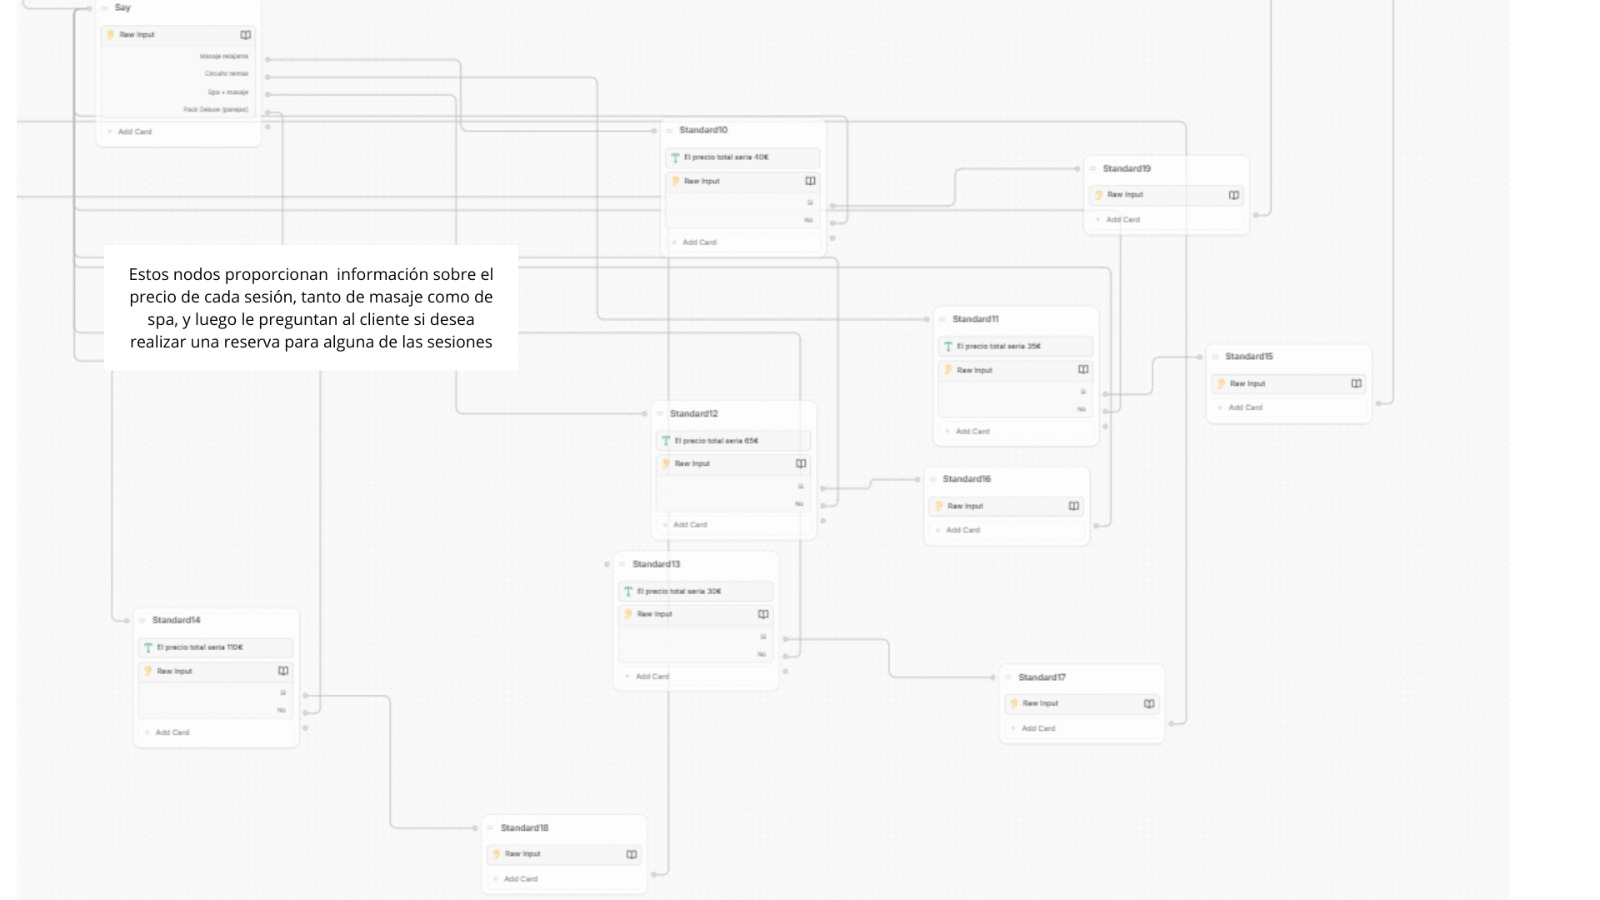
\includegraphics[width=.5\textwidth]{assets/workflow2.jpeg}
    \label{fig:my_label}
\end{figure}

El flujo continua con la gestión de reservas, donde el chatbot solicita información sobre la fecha de llegada, la fecha de salida, el número de personas
y el tipo de habitación deseado. Una vez recopilada esta información, el chatbot verifica la disponibilidad de habitaciones y confirma la reserva al usuario.

\begin{figure}[h!]
    \centering
    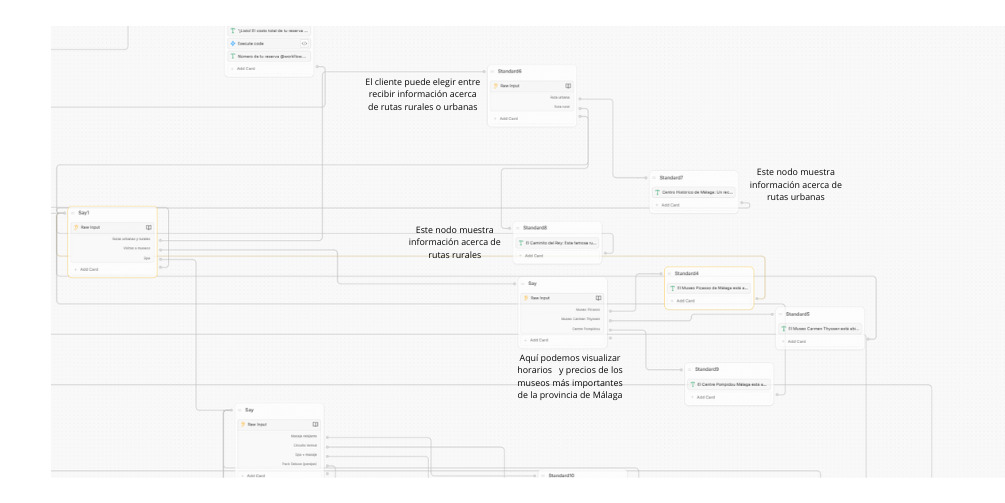
\includegraphics[width=.5\textwidth]{assets/workflow3.jpeg}
    \label{fig:my_label}
\end{figure}

Finalmente la recomendación de actividades y la resolución de problemas son dos nodos de decisión que permiten al chatbot ofrecer información adicional
o contactar con soporte humano si es necesario. Estos nodos permiten personalizar la interacción con el usuario y ofrecer respuestas más precisas.

\subsection{Variables del Chat}

Para mejorar la experiencia del usuario, el chatbot utiliza variables que almacenan información relevante durante la conversación. 
Entre estas variables se incluyen fechas de reserva, tipo de habitación, número de personas y lugar de preferencia. Más aún se puede
detallar problemas para reportarlos. Estas variables permiten al chatbot recordar información a lo largo de la conversación y ofrecer 
respuestas más personalizadas.

\begin{figure}[h!]
    \centering
    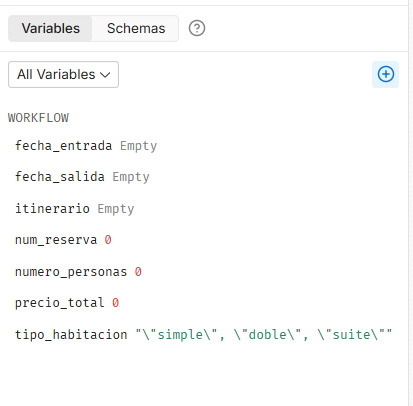
\includegraphics[width=.5\textwidth]{assets/Variables.jpeg}
    \label{fig:my_label}
\end{figure}

\clearpage

\section{Scripts}

Para la optimización del chatbot, se han desarrollado scripts y configuraciones específicas que permiten gestionar reservas, calcular precios y
proporcionar respuestas contextuales. Estos scripts se han integrado en el flujo conversacional y se ejecutan en función de las necesidades del usuario.

\subsection{Cálculo del Precio de la Reserva}

El siguiente script se encarga de calcular el precio total de una reserva en función de la fecha de entrada, la fecha de salida, el tipo de habitación
y el número de personas. El precio de la habitación se define en un objeto con los precios por tipo de habitación, y se calcula multiplicando el precio
por noche por el número de noches y el número de personas. El resultado se almacena en la variable workflow.precio\_total y se devuelve al usuario.

\begin{verbatim}

    const precioHabitacion = {
      simple: 80,
      doble: 120,
      suite: 200
    };
    
    //  Verificar que workflow está definido
    if (!workflow || typeof workflow !== "object") {
      throw new Error(" Error: El objeto 'workflow' no está definido o no es válido.");
    }
    
    //  Validar que los datos existen y son correctos
    if (!workflow.fecha_entrada || !workflow.fecha_salida || !workflow.tipo_habitacion || !workflow.numero_personas) {
      throw new Error(" Faltan datos para calcular el precio total.");
    }
    
    //  Asegurar que las fechas sean cadenas y convertirlas a Date
    if (typeof workflow.fecha_entrada !== "string" || typeof workflow.fecha_salida !== "string") {
      throw new Error(" Error: Las fechas deben ser cadenas en formato válido (YYYY-MM-DD).");
    }
    
    const fechaEntrada = new Date(workflow.fecha_entrada);
    const fechaSalida = new Date(workflow.fecha_salida);
    
    if (isNaN(fechaEntrada.getTime()) || isNaN(fechaSalida.getTime())) {
      throw new Error(" Las fechas ingresadas no son válidas.");
    }
    
    //  Calcular número de noches
    const noches = Math.ceil((fechaSalida.getTime() - fechaEntrada.getTime()) / (1000 * 60 * 60 * 24));
    
    if (noches <= 0) {
      throw new Error(" La fecha de salida debe ser posterior a la fecha de entrada.");
    }
    
    //  Validar y obtener el precio de la habitación
    const tipoHabitacion = workflow.tipo_habitacion.trim().toLowerCase();
    const precioPorNoche = precioHabitacion[tipoHabitacion];
    
    if (!precioPorNoche) {
      throw new Error(" El tipo de habitación ingresado no es válido.");
    }
    
    //  Validar y convertir el número de personas
    const numeroPersonas = parseInt(workflow.numero_personas, 10);
    if (isNaN(numeroPersonas) || numeroPersonas <= 0) {
      throw new Error(" Error: La cantidad de personas debe ser un número válido y mayor a 0.");
    }
    
    //  Cálculo del precio total
    workflow.precio_total = precioPorNoche * noches * numeroPersonas;
    
    console.log(" Precio total calculado:", workflow.precio_total);
    
    // Devolver el resultado
    return { totalReserva: workflow.precio_total };

\end{verbatim}

\subsection{Itinerario de viaje}

El siguiente script genera un itinerario de viaje personalizado para el usuario, basado en la fecha de entrada y la fecha de salida proporcionadas.
El itinerario incluye una lista de actividades recomendadas en Málaga, que se repiten en un ciclo para cubrir todas las noches de la estancia.

\begin{verbatim}

    //  Actividades recomendadas en Málaga por día
    const actividadesMalaga = [
    "Visita la Alcazaba y el Teatro Romano ",
    "Paseo por la Calle Larios y Plaza de la Constitución ",
    "Día de playa en La Malagueta ",
    "Tour por el Museo Picasso ",
    "Excursión a Mijas o Ronda ",
    "Ruta gastronómica por los mercados de Málaga ",
    "Día de senderismo en el Caminito del Rey "
    ];

    //  Verificar que los datos existen
    if (!workflow.fecha_entrada || !workflow.fecha_salida) {
    throw new Error(" Faltan datos para generar el itinerario.");
    }

    //  Convertir las fechas a formato válido
    const fechaEntrada = new Date(workflow.fecha_entrada);
    const fechaSalida = new Date(workflow.fecha_salida);

    //  Verificar si las fechas son válidas
    if (isNaN(fechaEntrada.getTime()) || isNaN(fechaSalida.getTime())) {
    throw new Error(" Las fechas ingresadas no son válidas.");
    }

    //  Calcular número de noches correctamente
    const noches = Math.ceil((fechaSalida.getTime() - fechaEntrada.getTime()) / (1000 * 60 * 60 * 24));

    if (noches <= 0) {
    throw new Error(" La fecha de salida debe ser posterior a la fecha de entrada.");
    }

    //  Generar itinerario personalizado
    let itinerario = [];
    for (let i = 0; i < noches; i++) {
    let actividad = actividadesMalaga[i % actividadesMalaga.length]; // Rotación de actividades
    itinerario.push(Día ${i + 1}: ${actividad});
    }

    //  Guardar en workflow para usar en Botpress
    workflow.itinerario = itinerario.join("\n");

    //  Mostrar en la consola (para debugging)
    console.log(" Itinerario generado:");
    console.log(workflow.itinerario);

    //  Devolver el resultado
    return { planViaje: workflow.itinerario };

\end{verbatim}

\section{Configuración}

\subsection{Prompts y Respuestas Contextuales}

El chatbot cuenta con diferentes prompts configurados para adaptarse a las respuestas del usuario. Mediante el uso de condiciones y reglas en Botpress, 
el chatbot es capaz de reformular preguntas o proporcionar información adicional según el contexto de la conversación. Esto garantiza una interacción 
fluida y natural con el usuario.

\begin{figure}[h!]
    \centering
    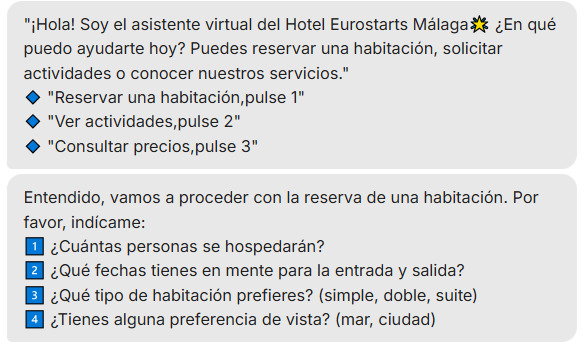
\includegraphics[width=.6\textwidth]{assets/Promts.jpeg}
    \label{fig:my_label}
\end{figure}

\subsection{Integración con Booking para la Verificación de Reservas}

Para comprobar la disponibilidad de habitaciones y gestionar reservas, el chatbot se integra con la API de Booking. Esta integración permite al chatbot 
verificar en tiempo real si una reserva existe, modificar reservas existentes o proporcionar detalles sobre una reserva específica. La conexión con 
Booking se ha logrado mediante la ejecución de consultas API desde los módulos de Botpress.

\begin{figure}[h!]
    \centering
    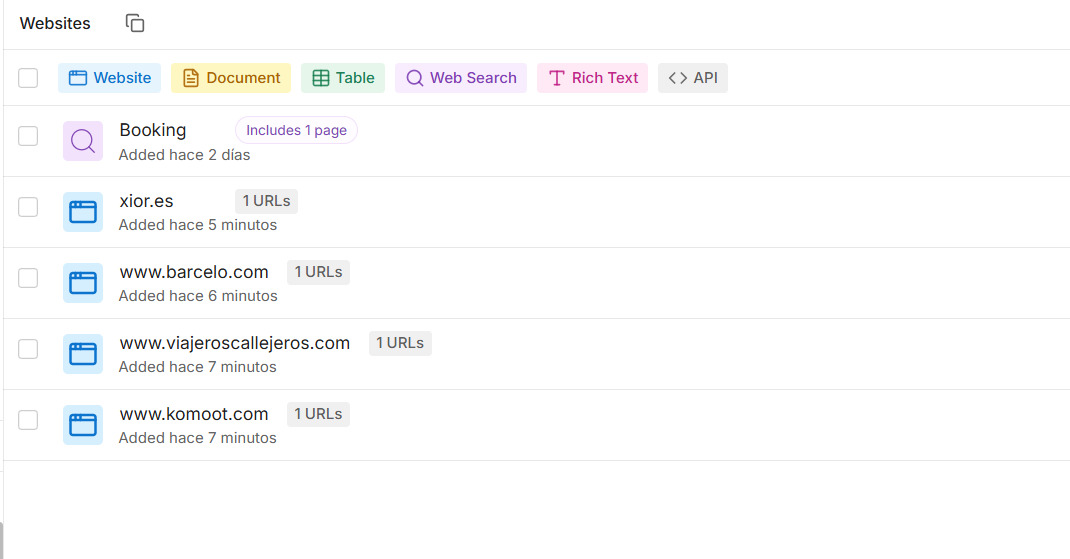
\includegraphics[width=.6\textwidth]{assets/apiBooking.jpeg}
    \label{fig:my_label}
\end{figure}

\section{Demostración del Chatbot}

Enlace para el chatbot: \href{https://cdn.botpress.cloud/webchat/v2.2/shareable.html?configUrl=https://files.bpcontent.cloud/2025/02/20/18/20250220181209-C0YQTWRL.json}{Hotel-Chatbot}

A continuación vamos a ver una serie de capturas de pantalla de la demostración del chatbot en acción.
Simulando la interacción con un usuario medio. (Nuestro chatbot a tenido un contratiempo Y
las fechas de las reservas hay que indicarlas en formato YYYY-MM-DD)

\begin{figure}[h!]
    \centering
    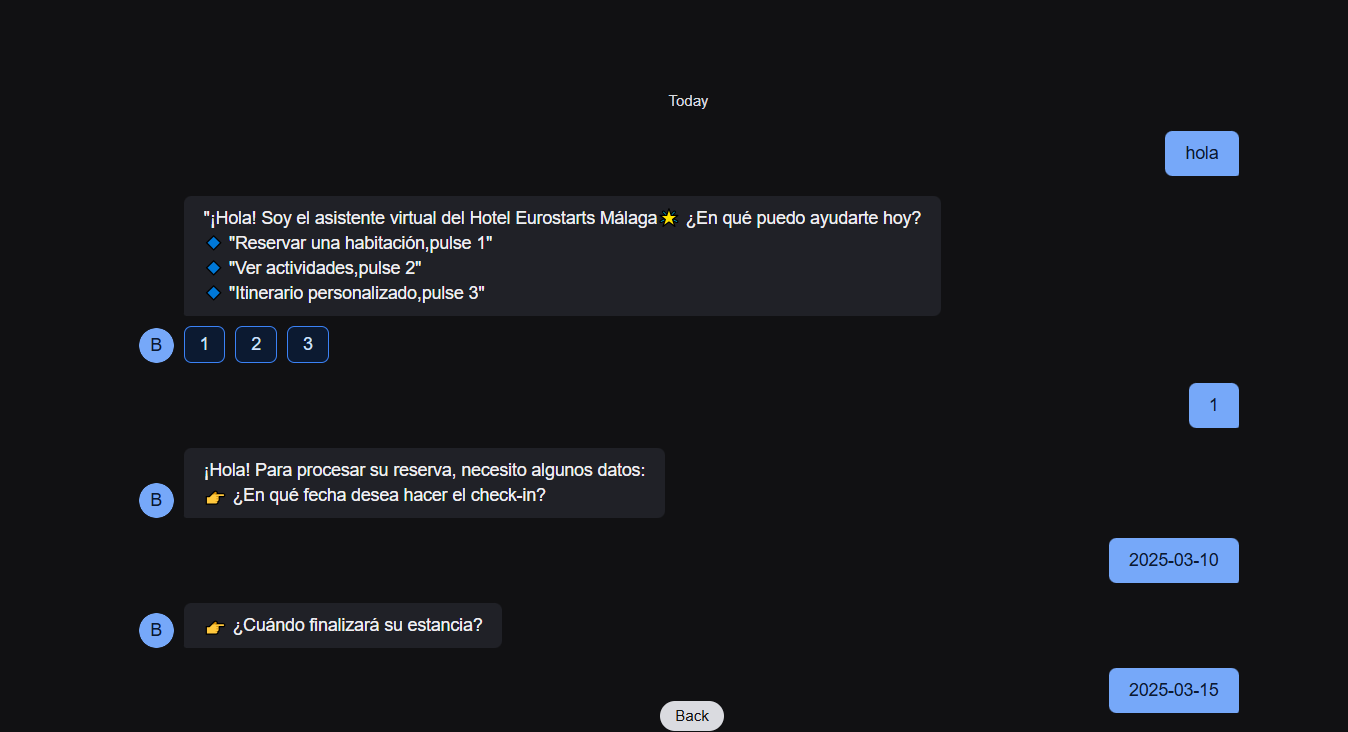
\includegraphics[width=.6\textwidth]{assets/ejemplo/conver-1.PNG}
    \label{fig:my_label}
\end{figure}

\begin{figure}[h!]
    \centering
    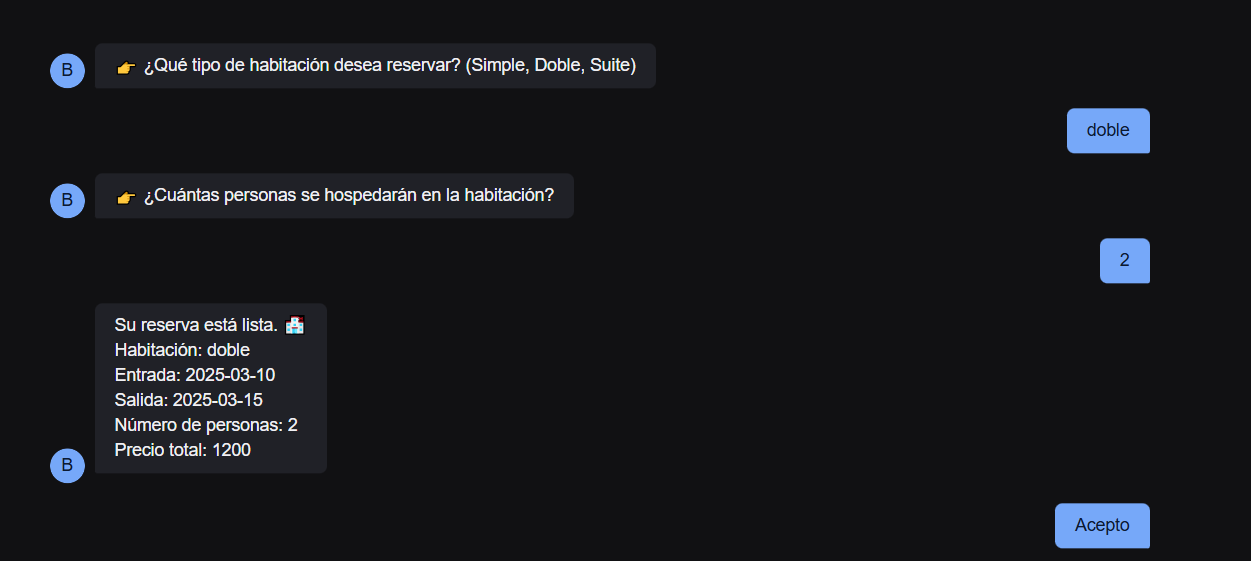
\includegraphics[width=.6\textwidth]{assets/ejemplo/conver-2.PNG}
    \label{fig:my_label}
\end{figure}

\begin{figure}[h!]
    \centering
    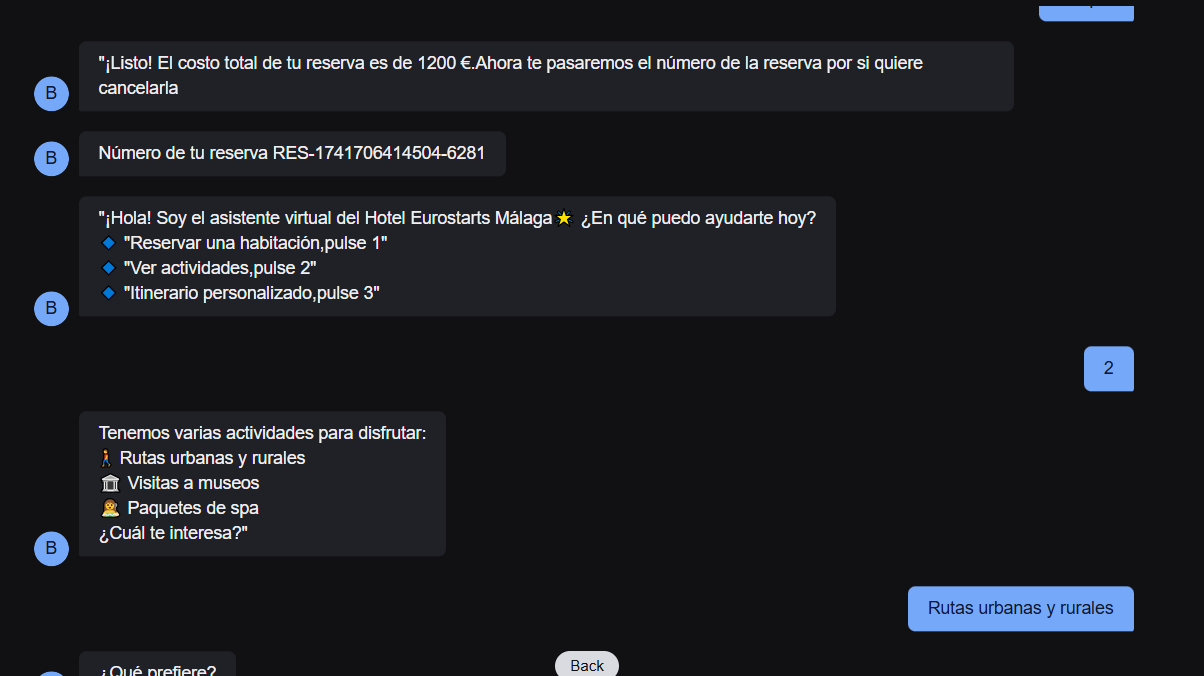
\includegraphics[width=.6\textwidth]{assets/ejemplo/conver-3.PNG}
    \label{fig:my_label}
\end{figure}

\begin{figure}[h!]
    \centering
    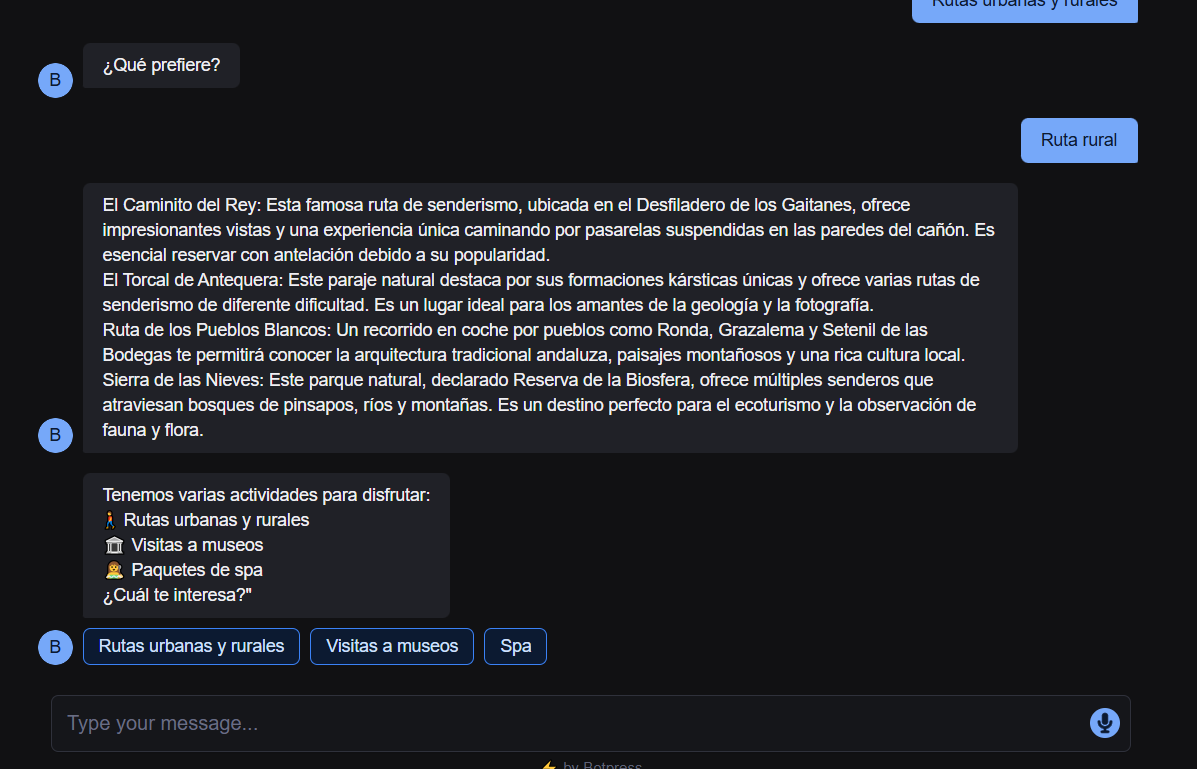
\includegraphics[width=.6\textwidth]{assets/ejemplo/conver-4.PNG}
    \label{fig:my_label}
\end{figure}

\begin{figure}[h!]
    \centering
    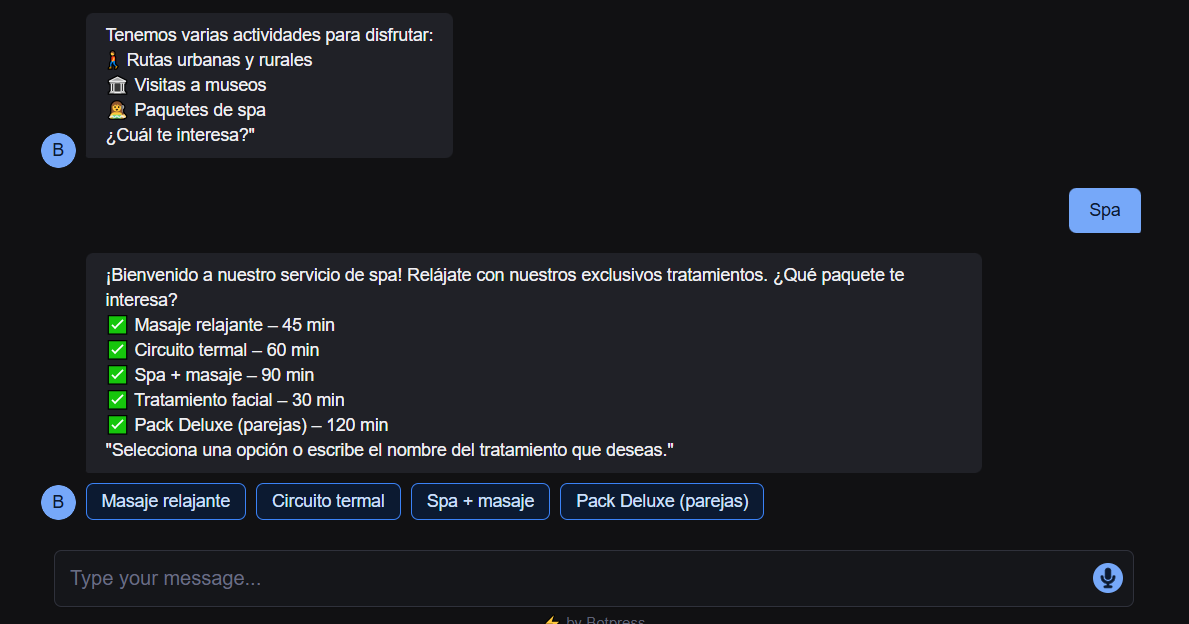
\includegraphics[width=.6\textwidth]{assets/ejemplo/conv-5.PNG}
    \label{fig:my_label}
\end{figure}

\begin{figure}[h!]
    \centering
    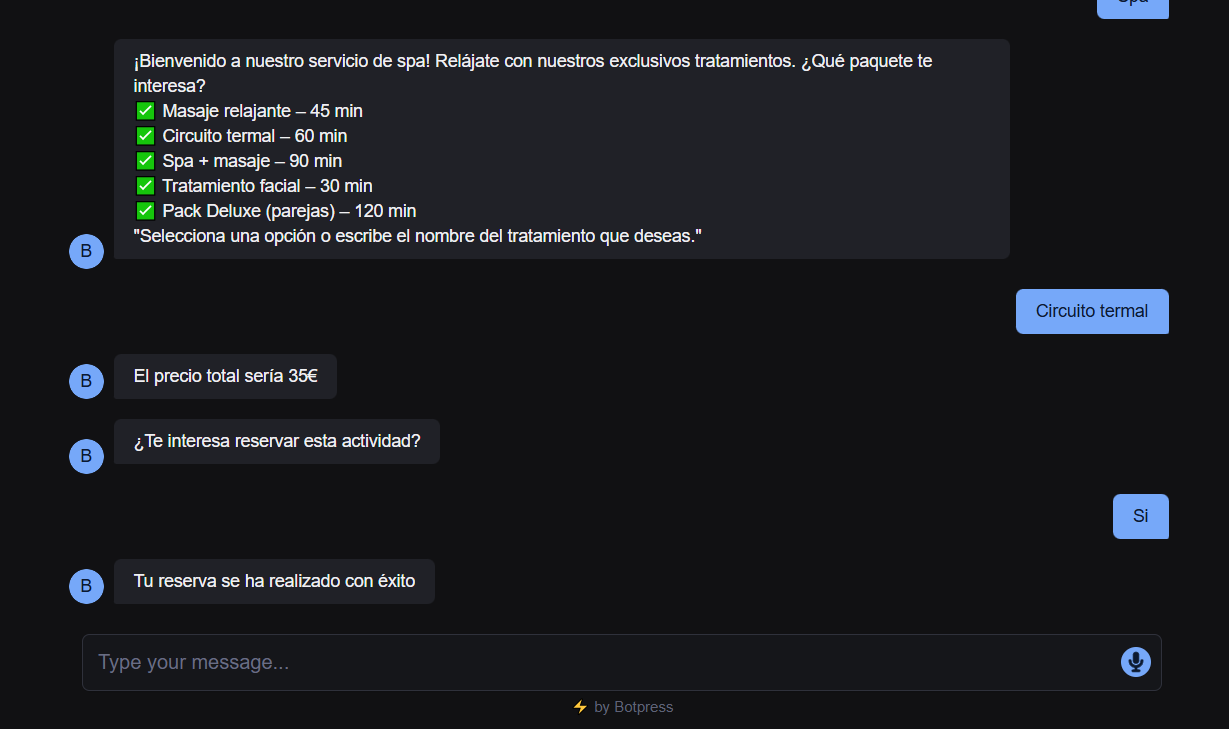
\includegraphics[width=.6\textwidth]{assets/ejemplo/conv-6.PNG}
    \label{fig:my_label}
\end{figure}

\clearpage

\section{Conclusión}

El desarrollo de un chatbot para asistencia hotelera en Botpress demuestra la capacidad de automatizar la atención al cliente de manera eficiente. 
Gracias a un workflow bien estructurado, el uso de variables, respuestas adaptativas y la integración con Booking, el chatbot es capaz de gestionar 
reservas, proporcionar asistencia y mejorar la experiencia del usuario en el hotel. Esta implementación no solo reduce la carga de trabajo del personal, 
sino que también mejora la satisfacción de los huéspedes al ofrecer respuestas rápidas y precisas.


\clearpage

\section{Bibliografia}

\cite{Botpress}

\printbibliography

\end{document}
